\section{Introduction}

\subsection{Lab and project objectives}

The objective of this project is to design an entire microcontroller system, that uses many common functionalities of a microcontroller. In this lab, we use the PSoC device from Cypress, but the skills that will be learned during this project should be applicable to different microcontroller families (DSPIC, STM32, ...). 

One important part of this project is for students to be able to browse through microcontroller documentation. To reach that objective, information and details about the PSoC microcontroller are purposely left out of this assignment, in order to force the student to find help in online and offline documentation. Teaching assistants can provide support for questions about system design, but will not help with questions that are related to implementation or coding of PSoC functionalities. 


\subsection{Available hardware}

In this project, you will dispose of the following hardware elements. 
\begin{itemize}
	\item An PSoC board (CY8CKIT-059) with a custom ULB-designed extension board (containing switches, a potentiometer, an audio jack output,  LEDs, ...). The details of the extension board can be found in the schematics at the end of this document; 
	\item two servomotors; 
	\item a photoresistor (i.e. a light probe); 
	\item a 2.7~k$\Omega$ resistor; 
	\item a keyboard; 
	\item a LCD screen (on the extension board); 
	\item a serial-to-USB converter to allow your computer to communicate over the serial port; 
	\item a small breadboard;  
	\item 15 male-male cables. 
\end{itemize}
The PSoC board is shown in Figure~\ref{fig:psoc}. It consist of the PSoC microcontroller (i.e. the integrated circuit in the center of the board) and a programmer (i.e. the integrated circuit on the left side of the board). The programmer allows to upload the program to the microcontroller directly from a host computer. Figure~\ref{fig:psoc} also show two pins that can be used to provide a 5~V and a GND signal (while allowing to provide some current) directly from the host computer USB port. 
\begin{figure}
	\centering
	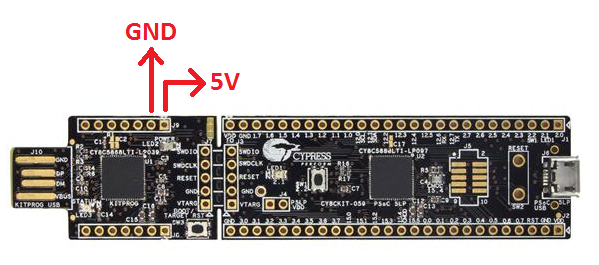
\includegraphics[width=4in]{psoc}
	\caption{PSoC boards. }
	\label{fig:psoc}
\end{figure}